%
% prinzip.tex -- Printzip der Lösung mit dem Euler-Verfahren
%
% (c) 2020 Prof Dr Andreas Müller, Hochschule Rapperswil
%
\documentclass[tikz]{standalone}
\usepackage{amsmath}
\usepackage{times}
\usepackage{txfonts}
\usepackage{pgfplots}
\usepackage{csvsimple}
\usetikzlibrary{arrows,intersections,math}
\begin{document}
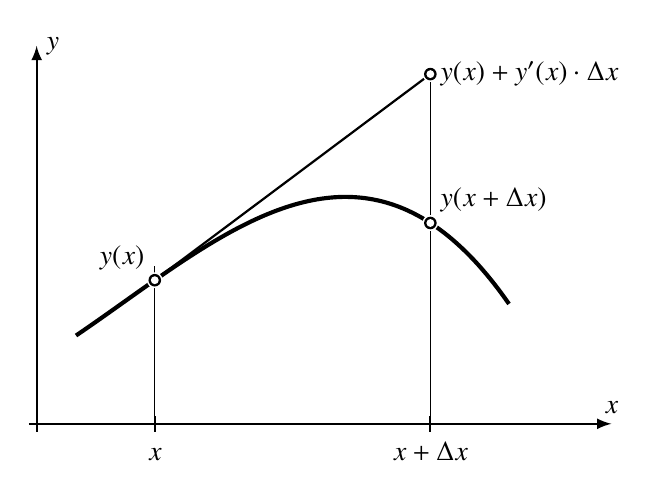
\begin{tikzpicture}[>=latex,thick]

\def\punkt#1{
	\fill[color=white] #1 circle[radius=0.1];
	\fill[color=black] #1 circle[radius=0.08];
	\fill[color=white] #1 circle[radius=0.05];
}

\def\x{5}

\def\A{-0.03}
\def\B{0.1}
\def\C{0.6}
\def\D{0.8}

\def\kurvenpunkt#1{({#1},{((\A*#1+\B)*#1+\C)*#1+\D})}
%({#1},{((\A*#1+\B)*#1+\C)*#1+\D})

% Ableitung
%({#1},{(3*\A*#1+2*\B)*#1+\C})

\draw[line width=1.5pt]  plot[domain=0.5:6,samples=100] (\x,{((\A*\x+\B)*\x+\C)*\x+\D});
%\draw plot[domain=0.5:6,samples=100] \kurvenpunkt{#1};

% Steigung
\pgfmathparse{((3*\A*1.5+2*\B)*1.5+\C)}
\xdef\m{\pgfmathresult}

\coordinate (E) at (0.5,0.5);
\coordinate (A) at ({1.5},{((\A*1.5+\B)*1.5+\C)*1.5+\D});
\coordinate (B) at (5,{((\A*5+\B)*5+\C)*5+\D});
\coordinate (C) at (5,{2+3.5*\m});
\coordinate (F) at (6,3.0);

\draw[line width=0.5pt] (\x,0)--(\x,4.5);
\draw (\x,-0.1)--(\x,0.1);
\node at (\x,-0.1) [below] {$\mathstrut x+\Delta x$};

\draw[line width=0.5pt] (1.5,0)--(1.5,2);
\draw (1.5,-0.1)--(1.5,0.1);
\node at (1.5,-0.1) [below] {$\mathstrut x$};

\draw (A)--(C);

\punkt{(A)}
\punkt{(B)}
\punkt{(C)}

% Punkte
\node at (A) [above left] {$y(x)$};
\node at (B) [above right] {$y(x+\Delta x)$};
\node at (C) [right] {$y(x)+y'(x)\cdot\Delta x$};

% Achsen
\draw[->] (-0.1,0)--(7.3,0) coordinate[label={$x$}];
\draw[->] (0,-0.1)--(0,4.8) coordinate[label={right:$y$}];

\end{tikzpicture}
\end{document}

